
\title{Ab initio methods for nuclear structure and reactions: from few to many nucleons}
\author{Giuseppina Orlandini} 
\institute{Giuseppina Orlandini \at Dipartimento di Fisica, Universit\`a di Trento, Via Sommarive, 14 I-38123 Trento, Italy,
Trento Institute for Fundamental Physics and Applications - I.N.F.N, Via Sommarive 14, I-38123 Trento, Italy, \email{giuseppina.orlandini@unitn.it}}
\maketitle

\abstract{These lecture notes intend to give a brief overview of some {\it ab initio} approaches currently used to study 
nuclear structure  properties and reactions.
In the first part particular attention is devoted to two methods useful to account for bound state properties. 
They are both based on the diagonalization of the full many-body Hamiltonian matrix, but share in addition 
the use of similarity transformations.
Transforming the bare potential into an effective one, the latter help in speeding up the convergence of the results.
In the second part {\it ab initio} methods for reaction cross sections involving 
the continuum part of the nuclear spectrum is described, with emphasis on perturbation induced reactions. 
They are based on integral transforms which make it possible to reduce 
the many-body scattering problem to a bound state problem, allowing to take advantage of any of the methods described in the first part.}


\section{Introduction: Theory, Model, Method}\label{sec:TMM}

The importance of studying nuclei lays in the fact that they are the most common manifestation of the strong 
interaction at {\it low}-energy (order of MeV), a regime where the fundamental theory, 
Quantum Chromo-Dynamics (QCD), is non-perturbative. 

Describing nuclei as an assembly of interacting  protons and neutrons corresponds to choosing the {\it effective} degrees 
of freedom (d.o.f) most relevant at that energy. This idea comes from observing that just protons and/or neutrons 
emerge, when energies of a few MeV are transferred to a nuclear system.
Since such degrees of freedom have a comparatively much larger mass (about one GeV), we are allowed 
to adopt a non relativistic quantum mechanical  framework to describe  nuclear  properties.
Then, any observable we would like to account for, will require solving the Schr\"odinger equation, 
governed by a many-nucleon Hamiltonian. In other words we will need to solve the so called {\it non relativistic quantum many-body problem}.

In this context we will adopt the word {\it Theory} referred excluvely to non relativistic quantum mechanics (NRQM), 
in Schr\"odinger, Heisenberg or Interaction representation. The word {\it \bf Model} will be used in connection to the choice
of the d.o.f. and of their mutual interaction, namely  the potential part of the Hamiltonian.
It is clear that any nuclear {\it  Model} (in the above acceptation) must have its roots in QCD, and that the Hamiltonian 
will have to share all its symmetries with QCD.  
These lectures will not deal with the problem of establishing the best {\it model} for a ``realistic'' potential 
(this subject is extensively treated elsewhere 
in this book), here we limit ourselves to consider it as an input for our problem. 

Summarizing, we want to calculate observables within our defined {\it Theory}, with an input nuclear {\it Model}, 
which is both rooted in QCD and {\it realistic} enough to accurately reproduce (at least) 
the nucleon-nucleon scattering data ($\chi$-square per datum close to 1).
However, in addition, we want to be able to control the degree of {\it accuracy} of the method used to solve 
the NRQM many-body problem, namely  we want to determine the theoretical accuracy on the value of an observable.
This is done by benchmarking different results obtained by different methods, using the same input.
All this is what characterizes an {\it ab initio} approach. Comparing the {\it ab initio} results to data we can 
learn about the degree of reliability of the nuclear {\it Model}. In this way we will be
able to predict new nuclear observables, as well as to give other fields (e.g. astrophysics) the needed nuclear information,
complemented by the degree of accuracy of the many-body method used.

\section{The Non-relativistic Quantum Mechanical Many-Nucleon Problem}\label{sec:NRQMP}

The non-relativistic quantum dynamics of a system of $A$ nucleons, supposed to have equal masses $m$,
is governed by the nuclear Hamiltonian $H$, 
which consists of kinetic energy $T$ and potential $V$:
\be
H = T + V  = \sum_{i=1}^A {\frac {{\p}^2_i} {2m} } + \sum_{i<j}^A V_{ij} + \sum_{i<j<k}^A V_{ijk} + ...\,.
\label{Hint}
\ee
In the equation above ${\p}_i$ is the momentum of the $i$-th nucleon in a general laboratory system,  
and $V_{ij}$ and $V_{ijk}$ denote the nucleon-nucleon (NN)
potential $V_{\rm NN}$, the three-nucleon potential $V_{\rm NNN}$, etc., respectively.
Notice that the reason why in general the nuclear Hamiltonian should contain many-body potentials is due to the fact 
the nucleons are {\it effective} degrees of freedom. The Chiral Effective Field Theory approach to the nuclear potential~\cite{EpM11}
 shows that nuclear forces obey a hierarchy: forces of
more and more many-body nature appear at higher and higher order in a perturbative expansion. 
In our discussion we will restrict to two- and three-body potentials, which appear to be the most relevant for common observables (in
general the inclusion of three-body potentials represents a technical challenge for most {\it ab initio} approaches).

Our problem consists in solving the Schr\"odinger equation,
\be
(H-E_n) |\Psi_n\rangle = 0 \,,
\ee
where $E_n$ and $|\Psi_n\rangle$ denote the eigenenergies and eigenfunctions of $H$, respectively.
The spectrum of $H$, represented by the infinite set of eigenenergies is discrete below, and continuous above, 
the first break-up threshold $E_{\rm th}$. 


In order to solve the Schr\"odinger equation  one has to supply proper
boundary conditions.  For $E < E_{\rm th}$ the wave function represents a bound state
and thus it is described by a square integrable (localized) function. This characteristic 
leads to major technical simplifications, compared
to the case  $E \ge E_{\rm th}$, where  the asymptotic boundary conditions pose   serious problems, especially when  $A>2$ 
(many-body scattering problem). 

There are different ways to tackle the NRQM problem for bound states or for the continuum. 
Very often a reformulation of the problem allows a practical solution, 
which seems impossible otherwise. It is this possibility that generates the richness of methods in many-body theory.



\subsection{Translation and Galileian Invariance}\label{sec:TGI}

A correct approach to the non relativistic many-nucleon problem  should fulfill 
two fundamental symmetries, namely those related to translational and Galileian invariance. One can easily show that the 
corresponding conserved quantities  are center of mass (CM) momentum 
$ {\P}_{CM} = \sum_i^A {\p}_i $ and CM position  $ {\R}_{CM} = \frac{1}{A}\sum_i^A {\r}_i $, respectively. 
Therefore the correct nuclear Hamiltonian must commute with those operators. This can be achieved if one rewrites  
Eq.~(\ref{Hint}) in terms of the Jacobi vectors, i.e. the $A$ independent (normalized) vectors  given by
$ {\R}_{CM}$ and  
%\be\label{jacobi}
%\bm{\eta}_{k-1}=\sqrt{\frac{k-1}{k}}\left({\r}_{k}-\frac{1}{k-1}({\r}_{1}+{\r}_{2}+...{\r}_{k-1})\right)\,\,\,\,\,\,\,k=2,3...A\,,
%\ee
\begin{eqnarray} \label{jacobi}
  \bm{\eta}_1 & = & \sqrt{\frac{A-1}{A}}\Big(\vec{ r}_1 
                - \frac{1}{A-1}(\vec{ r}_2 + \vec{ r}_3 + \cdots
                + \vec{ r}_{A} )\Big)  \nonumber \\
  \bm{\eta}_2 & = & \sqrt{\frac{A-2}{A-1}}\Big(\vec{ r}_{2} 
               - \frac{1}{A-2}(\vec{ r}_3 + \vec{ r}_4 + \cdots
               + \vec{ r}_{A} )\Big)  \nonumber \\
  &\ldots&  \nonumber \\ 
  \bm{\eta}_{N} & = & \sqrt{\frac{1}{2}}\Big( \vec{ r}_{A-1}
                        - \vec{ r}_{A} \Big) \,,\,\,\,\,\,\,\,\,\,\,\, N=A-1\,;
\end{eqnarray} 
together with their conjugate momenta ${\P}_{CM}$ and $\bm{\pi}_1, \bm{\pi}_2, ... \bm{\pi}_N$.

In terms of Jacobi vectors the Hamiltonian in (\ref{Hint}) becomes 
\be\label{Hlab}
H = H_{CM} + {\cal H} = \frac{\P_{CM}^2}{2 A m} + \sum_{i=1}^{A-1} \frac{\bm{\pi}_i^2}{2m} + V(\bm{\eta}_1,\bm{\eta}_2.... \bm{\eta}_{A-1})\,,
\ee
and the translation and Galileian invariant Hamiltonian of our interest is ${\cal H}$, which commutes both with $ {\P}_{CM}$ and 
$ {\R}_{CM}$.
An interesting remark is in order here:
any potential, even when it is limited to have a two-(or three-)body character, becomes an unseparated function of the $(A-1)$-coordinate 
in ${\cal H}$. 
This means that the system, when correctly expressed in terms of relative coordinates only, contains a correlation among the constituents, 
which goes beyond the dynamical one. One can call it a {\it CM correlation}. The latter  can be easily understood from the fact that
the movement of one particle will affect all the others, since the CM momentum and position remain fixed (conserved).

%A final remark on the notation:  in the rest of these notes the Hamiltonian denoted with H will always indicate the translational 
%and Galileian invariant  Hamiltonian 
%${\cal H}$ of Eq.~(\ref{Hlab}

\section{Classification of {\it Ab Initio} Approaches for Ground-state Calculations}\label{sec:CLASS}
As it was stated above the NRQM problem can be formulated in different ways. Therefore one can 
classify the {\it ab initio} methods in terms of just such different formulations, grouping them in different classes:
\begin{itemize} 
 \item  The Faddeev-Yakubowski (FY) method,
 \item  Methods based on the variational theorem,
 \item  Methods based on similarity transformations,
 \item  Quantum Monte Carlo methods.
\end{itemize}
In the following we will concentrate in particular on two of the methods rooted in the  variational theorem. However, in the following
a brief summary of the main peculiarities characterizing each group will be given. 
A more extensive description of the methods can be found in the quoted original references. A recent review can be found in~\cite{WlO12}. 
 
 \subsection{The Faddeev-Yakubowski (FY) Method}\label{sec:FY}
The very nice feature of the 
FY method is that it is formulated in a way that it is applicable to both bound and scattering states.
This method starts from the Lipmann-Schwinger (LS) reformulation 
of the Schr\"odinger equation and therefore deals with integral equations instead of differential equations. 
Today it is well known that a direct application of LS-type equations to the scattering problem for a system with more than two particles
does not lead to a unique solution. However, for quite some time  it was not clear 
how such a unique solution could be obtained. It was in 1961 that in his seminal work for the three-body system~\cite{FADDEEV:1961} Faddeev
showed how the problem can be solved. He derived the right set of coupled integral equations which
have taken his name: the Faddeev equations. 
Yakubowski~\cite{YAKUBOWSKY:1967} generalized the approach, in principle to any number of particles. However, 
the number of coupled equations to solve becomes prohibitive for more than four particles. 
 
A sort of variation of the FY equations are those introduced by Alt, Grassberger
and Sandhas (AGS equations)~\cite{AGS} who looked for possible further reductions of the FY problem. 
Assuming a separable form for the NN t-matrix leads to one-variable integral equations, which are much simpler 
to solve than the FY equations.

\subsection{Methods Based on the Variational Theorem (Diagonalization Methods)}\label{sec:VAR}
The diagonalization methods  are based on the Rayleigh-Ritz variational theorem~\cite{Ra870,Ri909}.
This theorem, which is very profitably applied every time  the solution of some useful equation renders stationary
some proper functional, finds a large application in quantum mechanics. In particular, one can show that the solution of the
Schr\"odinger equation (for a  state with finite norm) renders stationary  the energy
functional
\begin{equation}
 E[\Psi]=\frac{\langle\Psi|H|\Psi\rangle}{\langle\Psi|\Psi\rangle}\,.
\end{equation}

An important  lemma complements the fundamental variational theorem, stating that the value of the energy functional 
calculated with any trial function is always greater than the ground-state energy and equal to it, only when the trial function 
coincides with the exact ground-state wave function.
This means that one can find the ground state energy of a system by solving a minimization problem  
 \begin{equation}
 \delta E[\Psi]=0\,.\label{vareq}
\end{equation}

Numerous approaches use this variational principle to find the ground-state energy of a many-body system.
The approach is efficient if the trial function has a parametrized functional form that is both convenient 
and suitable to the problem to be solved. The various variational approaches differ by the choice of the trial function.
One very well known classical example is the Hartree-Fock method, where the trial function is a Slater determinant. 
In this case, however, it is not possible to give a theoretical estimate of how far the Hartree-Fock energy is from the correct result. 
Also the use of a parametrized functional form for the trial function and the minimization with respect to the parameters 
does not allow a theoretical  estimate of the error. More sophisticated approaches exist like the resonating group method~\cite{RGM1,RGM2}, 
where the trial function 
is chosen according to a cluster picture of the system  or the variational Monte Carlo (VMC) technique where the trial function reflects 
the form of the potential.

A more systematic approach consists in choosing the trial function $\Psi_T$ 
as an expansion on a complete (or over complete) set of square
integrable functions $\phi_n$ that respect the symmetries of the Hamiltonian:
\be
\label{Psi_trial}
|\Psi_T(N)\rangle = \sum_{n=1}^N c_n |\phi_n\rangle\,.
\ee
In this case the minimization procedure 
corresponds to finding the solution of a (generalized) eigenvalue problem 
\be
({\bf H}-E\,{\bf M})\,C=0 \,,\label{secular}
\ee
where $\bf H$ and $\bf M$ are $N \times N$ Hermitean matrices of the Hamiltonian ($H_{nm} = \langle \phi_n|  H |\phi_m\rangle$) 
and overlap integrals of the basis functions ($M_{nm} = \langle \phi_n|\phi_m\rangle$),
while $C$ represents the $N$-component vector formed by the linear parameters $c_n$.
With growing $N$ the size of the Hamiltonian matrix, 
represented on the chosen basis, increases and the true ground-state energy is approached from above. 
The basis can be complete as the hyperspherical harmonics (HH) or the harmonic oscillator (HO) basis,  or over-complete.
In principle the true result would be obtained only for an infinite number of basis functions, however,
the convergence of the smallest energy obtained after the diagonalization for large enough $N$ gives
the ground state energy. An estimate of the error can also be given, related to the convergence pattern.
One can  consider this as an  {\it ab initio} result. 

Here one should also mention another interesting variational method, namely the  stochastic variational method (SVM)~\cite{SVM1,SVM2}. 
Here again  the variational procedure does not proceed systematically 
by the diagonalization of a larger and larger Hamiltonian matrix,  
but in a stochastic way (trial and error), obtaining nevertheless rather good results when compared to other approaches~\cite{bench_2001}.

Variational approaches also allow to obtain the wave function corresponding to the minimal energy,
which can then be used to calculate other ground-state observables. However, one has to remember
that the difference between the exact value of the energy and that obtained with the trial function $\Psi_T$
which minimizes the energy functional, 
is an infinitesimal of higher order than the difference between the true wave function and $\Psi_T$. Therefore one should expect
a slower convergence and less accuracy for such observables.

\subsubsection{The Hyperspherical Harmonics (HH) Method}\label{sec:HH}

The HH method is a variational method where the trial function is written as
an expansion on the {\it hyper}-spherical harmonics (HH) basis. 
The HH are the generalization of the
spherical harmonics $Y_{lm}$. In fact as the latter represent a basis for the relative wave function of a two-body system,
the HH represent a general basis for the internal wave function of an $A$-body system.
Because of this,  they   are expressed in terms of the hyperspherical coordinates which are defined by a transformation 
of the Jacobi vectors.

Let us remember that the set of $A$ Jacobi vectors is composed 
by  $\R_{CM}$ and the $N=A-1$ relative vectors $\bm{\eta}_1,...,\bm{\eta}_N$ in Eq.(\ref{jacobi}), for a total of $3 A$ coordinates. 
The hyperspherical coordinates are defined by further transforming  
the $3N$ coordinates $\bm{\eta}_1,...,\bm{\eta}_N$ as follows:
the $2N$ polar angles $\theta_i$ and $\phi_i$ of the $\bm{\eta}_i\equiv(\eta_i,\theta_i,\phi_i)$ are left unaffected 
by the transformation. The remaining 
$N$  hyperspherical coordinates $\eta_i$ are expressed in terms of one {\it hyper}-radius $\rho_N$ and $(N-1)$ 
{\it hyper}-angles $\alpha_n$ defined by
\be
\sin\alpha_n= {\frac {|\eta_n|}{\rho_n}} \,; \,\,\,\,\,\,\,\,\,\,\,\,\,\,\rho^2_n  = \sum_{i=1}^n \eta_i^{\,2}
 \,, \,\,\, n=2,...,N \,.
\ee

A very interesting feature of the hyperspherical coordinates is that, when expressed in such coordinates,
the $A$-body kinetic energy operator of $A$ nucleons of equal masses is a sum of two terms ($\rho^2 \equiv \rho^2_N$)
~\cite{HiD56}
 \begin{equation}\label{Trho}
  T =  T_\rho + T_K(\rho)\,,\,\,\,\, {\rm with} \qquad T_\rho= - \frac{1}{2m}\Delta_{\rho} \,, \qquad 
T_K(\rho)=\frac{1}{2 m} \frac{{\bf K}_N^2}{\rho^2}\,,
\end{equation} 
namely it has a form which is  in perfect analogy to the three-dimensional case, 
with a {\it hyper}-radial dependent Laplacian $T_\rho$ and a {\it hyper}-centrifugal barrier $T_K(\rho)$.

The {\it hyper}-angular momentum operator ${\bf K}_N$ depends on all the $(3N-1)$ angles (denoted by 
$\hat\Omega_{[N]}$) and has a rather complicated form. But the main point here is that the HH 
are the orthonormal eigenfunctions ${\cal Y}_{[K_N]}(\hat\Omega_{[N]})$ of ${\bf K}_N^2$
\begin{equation}
{\bf K}_N^2\,{\cal Y}_{[K_N]}(\hat\Omega_{[N]})= K_N(K_N+3N-2){\cal Y}_{[K_N]}(\hat\Omega_{[N]})\,.
\label{eigeneqK2}
\end{equation} 
As one sees the eigenvalues are expressed in terms of the quantum number $K_N$. 
The subscript $[K_N]$ stands for the total set of $(3N-1)$ quantum numbers corresponding to commuting operators, namely
the hyperangular momenta ${\bf K}^2_N, {\bf K}^2_{N-1},... {\bf K}^2_2$ relative to the subsets of $N,N-1...2$ $\bm \eta$-coordinates, 
the angular momenta relative to each of the $N$ Jacobi coordinates $\vec l^2_N,\vec l^2_{N-1},...\vec l^2_1 $,
the total angular momenta $\vec L^2_N,\vec L^2_{N-1},...\vec L^2_2$ of the same subsets of $N,N-1...2$ $\bm \eta$-coordinates, 
and the third component of the total angular momentum $L^z$.
 
The ${\cal Y}_{[K_N]}(\hat\Omega_{[N]})$ are good  basis functions for the hyperangular part of the $A$-body internal 
wave function, however, one also needs good basis functions for the hyperradial part of the wave function.
A suitable choice are the orthogonal Laguerre polynomials, because of their exponential weight function, reproducing the 
correct asymptotic behavior of the wave function.

The basis obtained  by the product of Laguerre polinomials and HH is a translation invariant  CM ``correlated``  basis 
(all particles are connected to each other!) and
has good asymptotic conditions, therefore one can expect a faster convergence with respect to using a translation invariant HO basis. 
However, just because of the mentioned correlation, the basis presents big difficulties when coping with the Pauli
principle, a  problem also common to the translation invariant HO basis. 
Based only on intuition one can guess that permutations of particles will lead to different definitions 
of the Jacobi coordinates and consequently of the hyperspherical coordinates. It would be a miracle if the  HH would have 
definite permutational symmetries. And in fact they do not, but they possess different  components 
of the irreducible representations of the symmetry group $S_A$. Even when this problem is overcome 
(see~\cite{NOVOSELSKY:1994,BARNEA:1997+8, Gatto:2011,Deflorian:2013}), as the number of particles increases the convergence 
becomes rather slow.

In order to speed up the convergence two ways have been followed: the Correlated Hyperspherical Harmonics expansion (CHH)  and the 
Hyperspherical Harmonics expansion with Effective Interaction (EIHH). The latter will be explained in Section~\ref{sec:EIHH}. 
The main idea of the CHH approach consists in acting on the bare HH functions with a Jastrow
operator $\hat J$ embodying the short range correlation due to the repulsive part of the potential.
Such a repulsion leads to high momentum components in the wave function which is responsible for the 
slow convergence of the bare HH expansion. The correlation operator $\hat J$ takes the form
\begin{equation}
 \hat J={\cal S}\prod_{i<j}\sum_{s,t}f_{st}(r_{ij})P_{st}(i,j)
\end{equation}
where $P_{st}(i,j)$  are projection operators onto nucleon pairs $(ij)$ with spin $s$ and isospin $t$ and
${\cal S}$ is a particle symmetrization operator. This method has been applied only to A=3,4 systems, since the loss of orthonormality
of the CHH limits its efficiency. In fact calculating the matrix elements of the potential requires $3N$ dimensional integrals.
The reason why  this is not the case for the uncorrelated HH basis is explained in the following.

When expressed in HH coordinates the invariant Hamiltonian $\cal H$ is
\begin{equation}
 {\cal H}=   T_\rho + T_K(\rho) + V(\rho, \hat\Omega_{[N]})\,.
\end{equation}
However, supposing for simplicity that the potential has a two-body character $\sum_{i<j} V_{ij}$
(but the present argument can be easily extended to three-body potentials) its matrix element 
on antisymmetric functions will be the sum of $A(A-1)$ identical integrals 
with, say, $i=A$ and $j=A-1$. This means that $V$  will be a function only of the Jacobi vector $\bm{\eta}_N$, namely
$V(\sqrt{2}\rho \sin \alpha_N, \theta_N,\phi_N)$, 
the recursive  construction of the HH allows then to use the orthonormality condition 
of the ${\cal Y}_{[K_{N-1}]}(\hat\Omega_{[N-1]})$ and reduce the calculation of the matrix element of the potential 
to a (at most) four-dimensional integral, for any number of particles. When the orthonormality condition of the HH is lost, like in the 
CHH case, this is no longer true and one is left with 3N-dimensional integrals.


\subsection{Methods Based on Similarity Transformations~\label{sec:SIM}}
Another reformulation of the quantum mechanical many-body problem is based on the use of similarity
transformations~\cite{Ok54,CoK60,DaS64,SuL80}.
In this case one considers that the following mean value
\be
E_0 = \langle\Psi_0| H|\Psi_0\rangle \,,
\ee
where $|\Psi_0\rangle$ is the ground state  of the Hamiltonian $H$, 
is invariant under similarity transformations $e^S$, i.e.
\begin{equation} 
E_0= \langle\Psi_0|e^{-S} \,e^{S}\, H\,e^{-S} \, e^{S}|\Psi_0\rangle
\equiv \langle \bar\Phi|{\bar H} |\Phi\rangle\label{simileq} \, 
\end{equation}
with  
\be
|\Phi\rangle = e^{S}|\Psi_0\rangle \,, \qquad |\bar\Phi\rangle = e^{-S^\dagger}|\Psi_0\rangle \,,
 \qquad{\bar H} = e^{S}\,H\,e^{-S}\,.
\ee 

At this point one may consider a subspace P of the  Hilbert space  with  eigenprojector $\hat P$ given by 
\be
\hat P=\sum_{n=1}^N |\phi_n\rangle\langle\phi_n|\,, 
\ee 
where the $|\phi_n\rangle$ are eigenfunctions of some well known Hamiltonian (e.g. $H_{HO})$.
Indicating by $\hat Q=I-\hat P$ the corresponding eigenprojector on the  residual space, one can write Eq.~(\ref{simileq})
as 
\begin{equation}
E=\langle \bar\Phi|(\hat P + \hat Q){\bar H}(\hat P + \hat Q) |\Phi\rangle =
\langle \bar\Phi|\hat P{\bar H}\hat P+\hat P{\bar H}\hat Q+\hat Q{\bar H}\hat P+\hat Q{\bar H}\hat Q|\Phi\rangle\,.
\end{equation}
If  the following decoupling condition is satisfied
\begin{equation}
 \hat Q{\bar H}\hat P = \hat Q e^{S}\, H\,e^{-S}\hat P = 0\,,
\label{decoup}
\end{equation}
one has
\begin{equation}
E=\langle \bar\Phi|\hat P{\bar H}\hat P|\Phi\rangle\,.
\end{equation} 
This means that if one solves the decoupling equation (\ref{decoup}) it is possible, in principle, to determine $S$ and therefore
calculate $E_0$ as the mean value of the {\it effective} operator ${\bar H}$ on the P-space.  

Notice that, while in the {\it bare} Hamiltonian $H$ the operators may have  a two- or three-body nature, the  
{\it effective} operator ${\bar H}$ will be in principle an $A$-body operator. So, in general the operator $S$, 
which generates the similarity transformation, may be written as a combination of operators of any $n\leq A$-body nature. 
It is clear that in actual calculations one has to apply some restrictions on the number of these $n$-body
operators. In this respect the similarity transformation approach has been used in two ways: 
\begin{itemize}
 \item  in the so called Coupled Cluster (CC) method~\cite{Zab:1978,HJ:2004}  (discussed elsewhere in this book) 
 to calculate the ground state energies and radii of A-body nuclei ($n\leq 3$, known as CCSD and CCSDT);
 \item to construct effective two- or three- body potentials, as described in the next Section~\ref{sec:LS},
 in order to accelerate convergence in the variational diagonalization approaches using the  HO  
and the HH basis (see Sections~\ref{sec:NCSM} and~\ref{sec:EIHH}).
\end{itemize}


%In the first case one operates a restriction to a finite number of terms (2 or 3), but the sum can be systematically enlarged 
%in principle. In the second case   and ii) in the construction of effective interactions
%in order to accelerate convergence in the variational diagonalization approaches, in particular with the HO  
%and the HH basis (see Sections~\ref{sec:NCSM} and~\ref{sec:EIHH})  
%treated below).

\subsubsection{The Similarity Transformation Method for Effective Interactions}
\label{sec:LS}
%The approach that is chosen to construct the effective Hamiltonian, and consequently the effective interaction, 
%appropriate to the finite P${\!_A}$-space, 
%is that described in Section~\ref{sec:SIM}. However, 

As was stressed in the previous Section, the similarity transformation leads to  an  effective Hamiltonian 
which is an $A$-body operator. To avoid this complication, an approximation is made. It consists 
in first finding only a two-body effective interaction $\tilde V_{ij}^{\rm [2,eff]}$
which is then used to replace  the {\it bare} interaction term $ V_{ij}$. This approach is often referred to
as the Lee-Suzuki (LS) method~\cite{SuL80}. The effective interaction $V_{ij}^{\rm [2,eff]}$
is obtained  by applying the decoupling condition of Eq.~(\ref{decoup}) to a two-nucleon
Hamiltonian $H^{[2]}$  that arises from ${\cal H}$ by restricting  the kinetic and potential operators
to two nucleons only (e.g. $i=A$ and $j=A-1$). In this simple case the decoupling condition can be solved.
In fact the two-body problem can be fully solved and in this case one has the knowledge of both the $P$ and the $Q$ sapce.

Once the effective interaction $ V_{12}^{\rm [2,eff]}$ is obtained one replaces it in the $\sum_{i<j} V_{ij}$.
The replacement in the potential term of the effective interaction $ V_{ij}^{\rm [2,eff]}$ 
makes the approach no longer  variational. 
The $n$-body terms neglected in the full effective Hamiltonian, could either increase
or decrease the binding energy. On the other hand, one has an important result: as the P${\!_A}$-space  is increased
the result has to converge to the exact solution.
This may be illustrated in a pictorial way as in Fig.~\ref{fig:1}. At each P$_{\!A}$,  since
the similarity transformation transfers information from the Q$_{2}$ space
to the P$_2$ space, there is much less information left out. Consequently the convergence on $E_0$ is much faster. 
When  P$_{\!\!A}$ is  sufficiently large, so that it covers almost the 
whole Hilbert space, the effective interaction practically coincides  with the bare one, and one has an accurate result. 
From the figure one can infer that the exact result could be reached also applying the similarity transformation to the 
three-body and then four-body  Hamiltonian etc., namely sistematically applying the similarity transformation to
move the information from the larger $Q_3$ space into the
$P_3$ space, from the $Q_4$ space into the $P_4$ space, etc..

However, this is much more problematic and  impossible in practice, since one would need to
know the entire $n$-body spectrum to construct the $n$-body effective interaction. 
Of course if three-body forces are present in the original Hamiltonian one has 
to apply the  procedure at least up to $n=3$.  
\begin{figure}
\sidecaption
% Use the relevant command for your figure-insertion program
% to insert the figure file.{\pi}
% For example, with the option graphics use
\includegraphics[scale=.65]{Chapter7-figures/fig1.eps}
%
% If not, use
%\picplace{5cm}{2cm} % Give the correct figure height and width in cm
%
\caption{The various P and Q spaces relevant for the construction
of the two-body effective interaction (see text).}
\label{fig:1}       % Give a unique label
\end{figure}

\subsection{Monte Carlo Methods}\label{sec:MC}

The Monte Carlo (MC) methods are based on a formulation of the quantum mechanical many-body problem
which is suited to a stochastic approach.  These methods are
the Green's Function MC (GFMC)~\cite{Ka62},  Diffusion MC (DMC)~\cite{Ca87} and Auxiliary Field Diffusion MC (AFDMC)~\cite{ScF99}, 
the Chiral Effective Field Theory on a Lattice (LCEFT)~\cite{Le09},
the Monte Carlo Shell Model Diagonalization (MCSMD)~\cite{KoD97,HoM95,OtH01}, 
and the Variational Monte Carlo (VMC)~\cite{PiW01}. 
The GFMC, DMC and AFDMC methods are based on the path integral formulation of quantum mechanics
(there are small differences between the GFMC and DMC methods so that in the literature they are often interchanged).
The LCEFT is  a DMC approach, except that the dynamical degrees of freedom are nucleon and pion fields rather than particles.
Both GFMC and LCEFT methods are based on the Euclidean time (imaginary time) evolution of the system.  
The MCSMD, although inspired by the imaginary time formulation, is  effectively a variational method. 
Starting from an  imaginary time evolved trial function,  after some manipulation,  MCSMD leads to an expression that suggests 
a way of constructing a variational shell model basis. In this case the imaginary time is just one of the non-linear parameters.
The  VMC method is a fully variational method. Here the MC technique is used to evaluate 
the many-dimensional energy functional integrals. The variational wave function  obtained with this method  
usually serves as starting trial function for the GFMC imaginary time evolution.

An extensive treatment of   Monte Carlo approaches can be found elsewhere in this book.

\section{Two Diagonalization Methods with Effective Interactions}\label{sec:TWOEI}

In this section we will describe two diagonalization methods, which have much in common: the No Core Shell Model (NCSM) 
and the Effective Interaction Hyperspherical Harmonic (EIHH) methods. They  both make use of the LS similarity transformation method  
 (see Section \ref{sec:LS}), in order to speed up the convergence. 
They differ only by the choice of the basis on which the Hamiltonian is diagonalized and, 
for $A > 4$, also for the way they treat translation invariance. 

\subsection {The No Core Shell Model Method (NCSM)}\label{sec:NCSM}
The name NCSM means that all the nucleons  are taken into
account  explicitly as degrees of freedom, namely  it is not assumed that there is an inert core, like in the traditional shell model. 
The NCSM couples the  advantage of the shell model (i.e. working in a HO basis) with the accuracy of an {\it ab initio} approach.  

In the literature two versions of the NCSM exist , which differ in the treatment of translation invariance.
In one version, the Hamiltonian of Eq.~(\ref{Hint})
is modified~\cite{ShF74} by adding a harmonic oscillator CM Hamiltonian $H_{\rm CM}$ to the intrinsic Hamiltonian $\cal H$
 \begin{eqnarray}
H^{[A]}_\Omega &=& {\cal H} + H_{\rm CM}^{\rm HO} = {\cal H} +  \frac {{\P}_{\rm \rm CM}^2} {2Am} + 
{\frac{Am}{2}} \Omega^2 {\bf R}_{\rm CM}^2 \\
\label{prova}
 &=& \sum_{i=1}^A \left[ {\frac{{\bf p}_i^2}{2m}}
+\frac{1}{2}m\Omega^2 {\bf r}^2_i
\right] + \sum_{i<j=1}^A \left[ V_{ij}
-\frac{m\Omega^2}{2A}
({\bf r}_i-{\bf r}_j)^2 
\right]\\
&\equiv& \sum_{i=1}^A h_i^{\rm HO} + \sum_{i<j=1}^A\tilde V_{ij} \,,
\label{HOmega}
\end{eqnarray}
where $\tilde V_{jk}$ is a modified potential which depends  on  both the HO frequency $\Omega$ and the nuclear 
system via the mass number $A$: 
\be
\label{Vtilde}
\tilde V_{ij}=\left[ V_{ij}
-\frac{m\Omega^2}{2A}
({\bf r}_i-{\bf r}_j)^2\right]\,.
\ee
Of course the added center of mass HO term has no influence on the internal motion. 
Therefore the ground-state energy $E$ of ${\cal H}$ is obtained
by subtraction of the CM ground-state energy $3\hbar \Omega/2$ from the ground-state energy 
$E^{[A]}_\Omega$ of $H^{[A]}_\Omega$. 

In order to obtain an accurate result the calculation of $E^{[A]}_\Omega$  should be  performed with the $\tilde V$ of Eq.(\ref{Vtilde})
in a finite model space  P${\!_A}$ spanned
by all the $A$-body HO Slater determinants formed by filling the single-particle HO eigenstates
with $N\leq N_{\rm max}$ ($N$ is the total number of single-particle HO quanta) and increasing  
P${\!_A}$, namely $N_{\rm max}$, up to convergence. However, since the convergence is very slow one can speed it up
using a $\tilde V^{\rm [2,eff]}$. This is obtained as described in Section.~\ref{sec:LS}, namely applying the SL procedure
to a two-body internal Hamiltonian obtained from (\ref{prova}) 
by restricting the sums to two nucleons only (e.g. nucleons $A$ and $A-1)$, keeping however the original mass number $A$ 
in the interaction term $\tilde V$:

\begin{equation}\label{HO2mega}
{\cal H}^{[2]}_\Omega = \left[ \frac{\bm {\pi}^2}{2 m}
+\frac{1}{2}m\Omega^2 \bm {\eta}^2\right ]+
\tilde V_{A(A-1)}
\equiv {\cal H}^{[2]}_{\rm HO} +\tilde V_{A(A-1)}  \,.
\end{equation}

 
%\begin{eqnarray}
%{\cal H}^{[2]}_\Omega &=&  \frac{{\bf p}_1^2}{2m}+\frac{{\bf p}_2^2}{2m}
%+\left[\frac{1}{2}m\Omega^2 {\bf r}^2_1+\frac{1}{2}m\Omega^2 {\bf r}^2_2
%\right] 
%+  \left[ V_{12}
%-\frac{m\Omega^2}{2A}
%({\bf r}_1-{\bf r}_2)^2\right]
%\equiv H^{[2]}_{\rm HO} +\tilde V_{12}  \,.
%\label{HO2mega}
%\end{eqnarray}

The effective Hamiltonian ${\cal H}^{[2]}_{\rm eff}$ is determined in  
the P$_{2}$-space ($\hat P_2+ \hat Q_2 =I_2$), a subspace of $P$, via 
the two-body transformation operator $S^{[2]}=\hat Q_2 S^{[2]}  \hat P_2$. 
Then by subtracting ${\cal H}^{[2]}_{\rm HO}$ from ${\cal H}^{[2]}_{\rm eff}$ the two-body effective interaction is obtained  i.e. 
\begin{equation}
\tilde V_{12}^{[2,\rm eff]}  = {\cal H}^{[2]}_{\rm eff} - {\cal H}^{[2]}_{\rm HO}\,.
\end{equation}
The obtained  $\tilde V_{ij}^{[2,\rm eff]}$  is then used in Eq.~(\ref{HOmega}).
As is clear from Ref.~\cite{DaS64}, this procedure 
is equivalent to  {\bf (i)} limiting the similarity operator $S$ of Section~\ref{sec:SIM}   to
a  two-body operator $S^{[2]}$ and {\bf (ii)} truncating the effective Hamiltonian   at the two-body operator level. 
When the diagonalization of the Hamiltonian is performed with the two-body effective interaction the  NCSM is no longer  variational. 
In fact, as was already stated above the real effective interaction obtained by a full similarity transformation at a fixed P-space
is an $A$-body interaction. The neglected $n>2$-body terms  could either increase
or decrease the binding energy. However, as the P-space increases
the result converges to the exact solution, as was already discussed in Section~\ref{sec:LS}. 

Another version of the NCSM exists~\cite{NAV:1998}, where the problem is  formulated directly in terms of Jacobi coordinates 
and the $A$-body basis is 
the translationally invariant HO basis.  However, it is  restricted to $A=3,\,4$, 
because of the same complications generated by the Pauli principle, as those was mentioned in Section~\ref{sec:EIHH}.


\subsection{The Hyperspherical Harmonics Method with Effective Interaction (EIHH)}\label{sec:EIHH}

The idea is very similar to that of the NCSM approach, but with the following two differences:
one is that the P-space is defined by a maximal value $K_{\rm max}$ of the 
grand angular quantum number $K_N$ ($N=A-1$), and the second is that 
the EIHH two-body Hamiltonian  undergoing the similarity transformation, $H_A^{[2]}$, is a {\it quasi} 
two-body Hamiltonian, because it  contains information about the dynamics of the entire $A$-body system via an hyperradial dependence. 
\begin{figure}
\sidecaption
% Use the relevant command for your figure-insertion program
% to insert the figure file.{\pi}
% For example, with the option graphics use
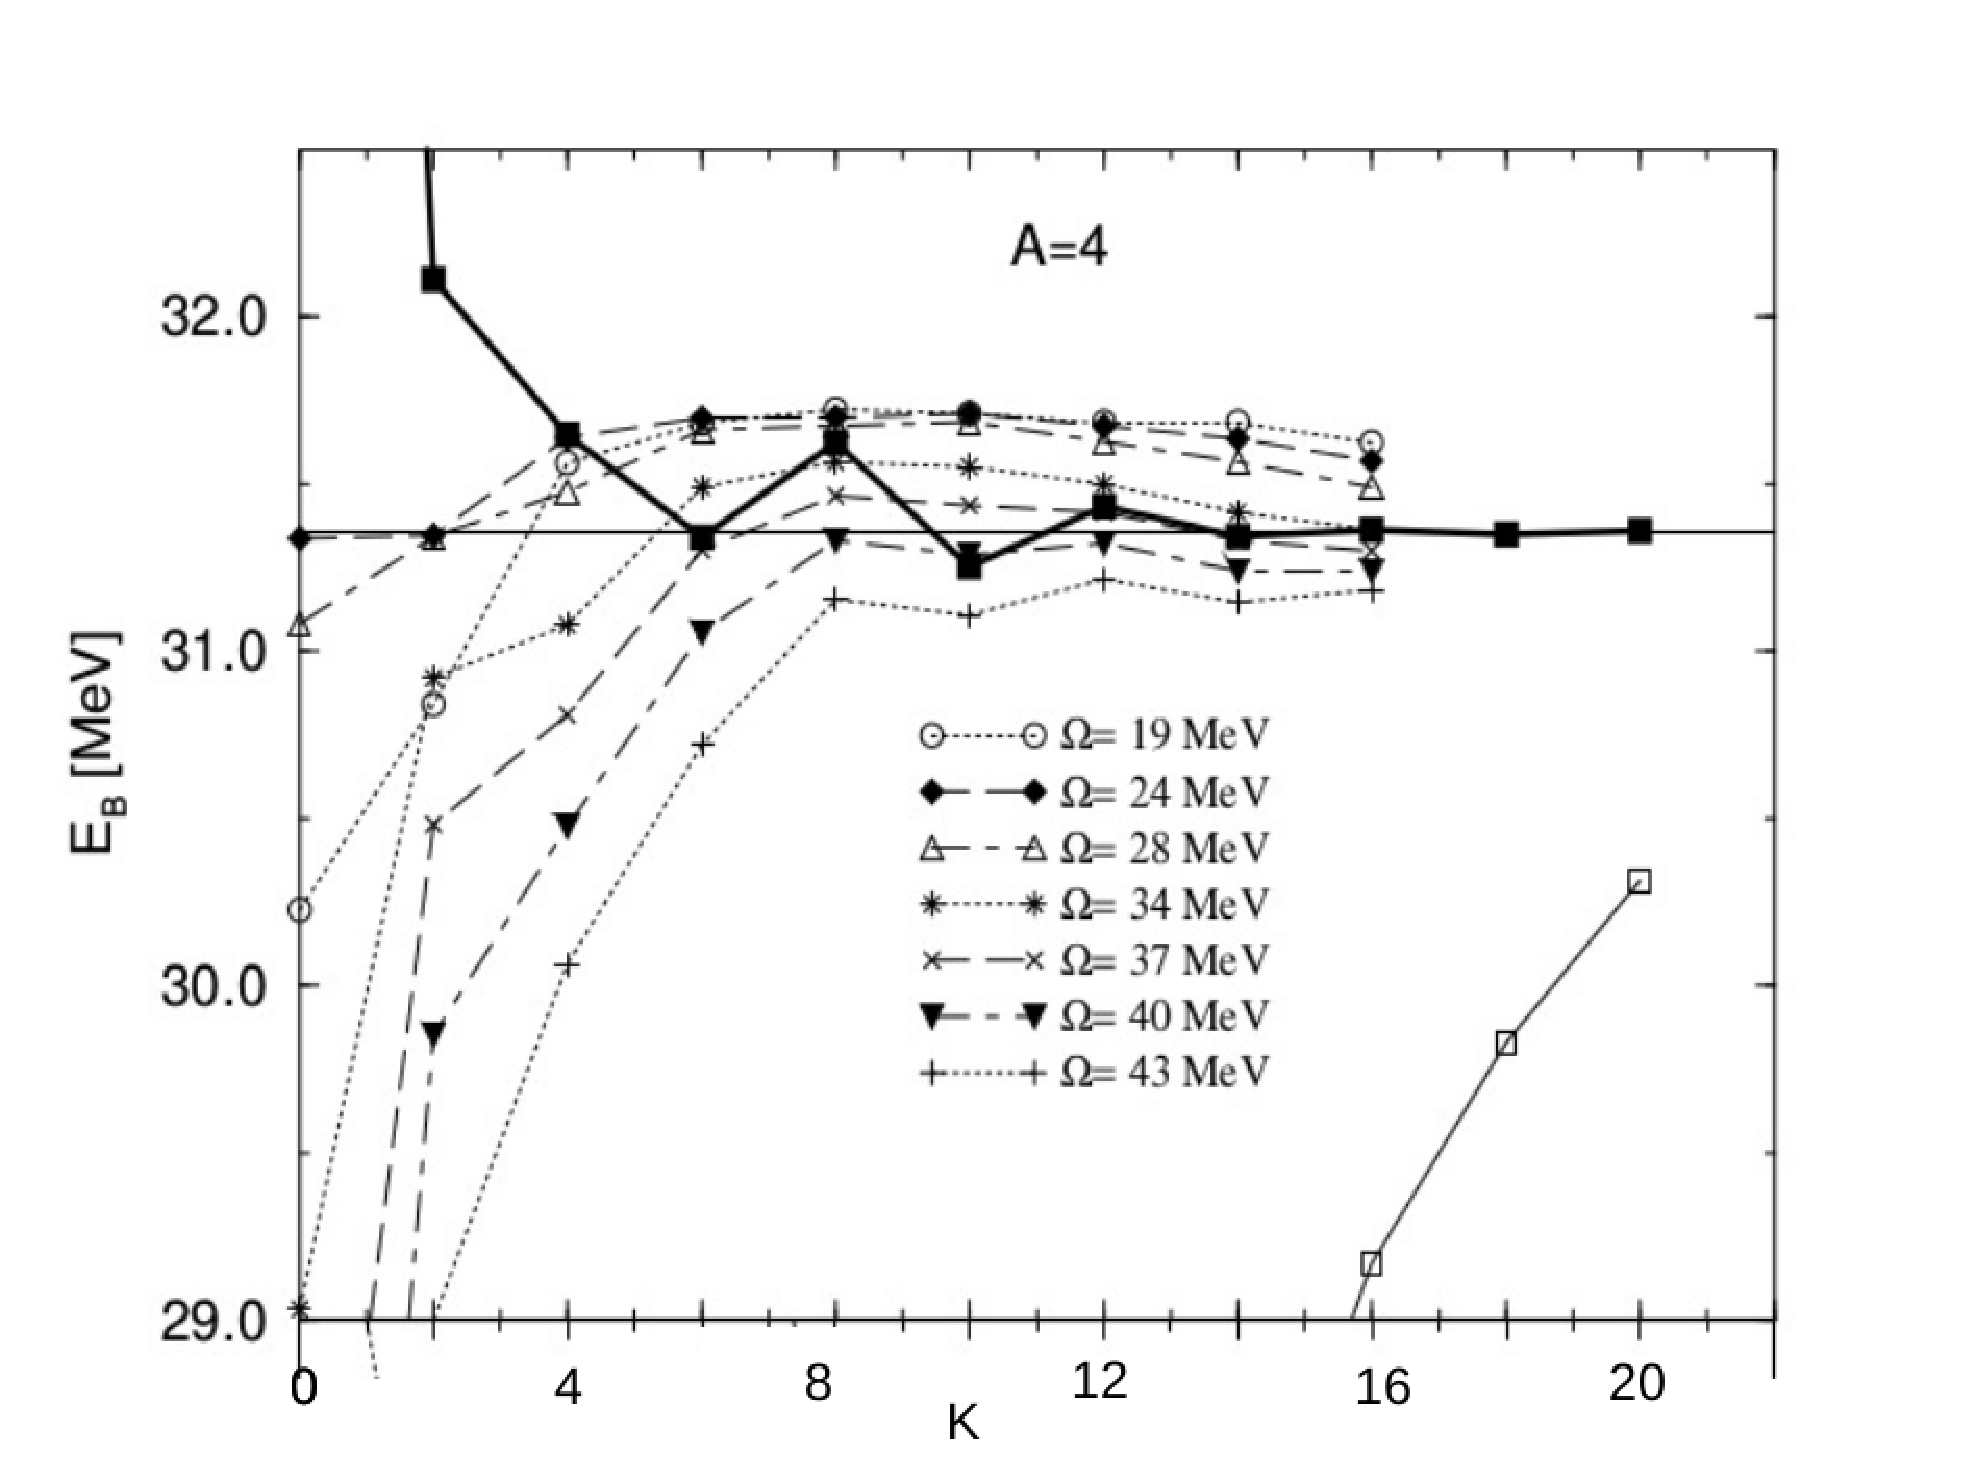
\includegraphics[scale=.35]{Chapter7-figures/fig2.eps}
%
% If not, use
%\picplace{5cm}{2cm} % Give the correct figure height and width in cm
%
\caption{Comparison between EIHH (full squares), pure HH 
(open squares)  and NCSM results obtained with different values of the HO
parameter.}
\label{fig:2}       % Give a unique label
\end{figure}

To be more explicit, the HH {\it quasi} two-body Hamiltonian is chosen as  
\begin{equation}
\label{H_quasi}
 H^{[2]}_A(\rho)= T_K(\rho) + V_{A,A-1}(\sqrt{2}\rho \sin{\alpha_N} \, \theta_N,\phi_N)\,,
\end{equation} 
where $T_K(\rho)$ is the collective hyperspherical kinetic energy of the entire $A$-body system 
(see Eqs.~(\ref{Trho})) and we make explicit only the spatial dependence of $V$ on two particles 
(chosen to be $A$ and $A-1$, consistent with  Jacobi coordinates constructed  in normalized reversed order, like those
in Eq.(\ref{jacobi}. 

The  transformation is applied separately for each value of the hyperradius $\rho$,
therefore the effective interaction becomes a function of $\rho$.
In addition to its $\rho$-dependence, the HH effective interaction
also depends on some quantum numbers of the
residual system. The  additional many-body information contained in the HH effective interaction 
(obtained by subtracting the hypercentrifugal term) is responsible for 
leading to a fast convergence of the HH expansion as can be seen in an example reported in Fig.~\ref{fig:2} from~\cite{BaL00}.
In this figure the binding energy of $^4$He was obtained using a central NN potential. One can notice the enormous advantage 
in the convergence pattern of the EIHH results in comparison to the HH ones. It is also interesting to notice the comparison with the NCSM 
results, which are spread around the EIHH one, depending on the HO parameter, as well as the non-variational behavior 
of the convergence pattern.


\section{Excited States}\label{sec:EXCITED}
%While with the FY method   
%the calculation of a discrete excited state follows the same line as that of the ground state  the situation is different 
%for the diagonalization approaches.
By diagonalizing the Hamiltonian matrix on a given finite basis of square integrable functions one gets a spectrum of $N$
eigenstates $\Psi_i$ with eigenvalues $E_i$. If the trial function has the same quantum numbers of the ground state
of the nucleus,  the lowest $E_i$ corresponds to the ground-state energy. The other solutions correspond to discrete excited 
states of the system, 
with the same quantum numbers as the ground state. Getting convergence for the energy of such excited states requires 
in general larger matrices. 
To find discrete excited states with quantum numbers different from those of the ground state one has to implement 
the proper quantum numbers into the basis set.

Few-nucleon systems have very few, if any, discrete excited states, in fact most of them lie 
in the continuum. Continuum eigenvalues 
are larger than the threshold energy $E_{th}$, corresponding to their ground state energy plus
the nucleon separation energy (the proton separation energy 
is always smaller than that of a neutron if the Coulomb force is considered). 
The  energy states larger than $E_{th}$ obtained by diagonalization do not have the proper 
continuum boundary conditions. 
Proceeding in such a way one obtains a fake discretization of the continuum. 

In order to avoid finding the continuum solutions of the Schr\"odinger equation, corresponding to 
solve the many-body scattering problem,
one can try again to reformulate the quantum mechanical problem in an accessible way.
This will be done in the next sections,  referring in  particular to observables that require the knowledge  of such continuum states.

\subsection{Response Functions to Perturbative Probes}\label{sec:RPP}

Here we focus on a particular family of reactions involving states in the continuum: we deal with nuclear reactions on light systems 
induced by perturbations. Typical examples are electroweak (e.w.) reactions like electron or neutrino scattering on nuclei or 
nuclear photabsorption.

The strength of the interaction Hamiltonian $H_{int}$ between an electromagnetic or weak probe and the nucleus is very weak when
compared to the strong interaction among the nucleons. Therefore the cross section can be calculated in first order 
perturbation theory, using the 
Fermi Golden rule. This means that the cross section will contain the transition rate proportional to the square modulus of the 
matrix element $ |\langle f|H_{int}|i\rangle|^2$ with $|i\rangle$ and $|f\rangle$ the initial and final states of the nucleus, 
as well as an energy conserving $\delta$-function
\begin{equation}
 \sigma\propto|\langle f|H_{int}|i\rangle|^2 \delta(\omega-E_f+E_i)\,,
\end{equation}
where $\omega$ is the energy transferred by the probe to the nucleus $(\hbar=c=1)$ and $E_f,E_i$ are the energies of the nuclear 
final and initial states, generally the ground state $|0\rangle$ and one of its $|n\rangle$ eigenstates (we suppose 
that in $\omega$ the  energy 
that has served to recoil the nucleus has been subtracted). 
In general the interaction $H_{int}$ can be described as the product of the ''current`` densities inside the nucleus  
and the field generated  by the probe, e.g. the charge density $\rho(\vec r)$ and the electromagnetic scalar potential $\varphi(\vec r)$
generated by the electrons in an electron scattering experiment
\begin{equation}
 H_{int}=\int d\vec r\,\rho(\vec r)\,\varphi(\vec r)
\end{equation}
In this example the nuclear  charge density is due to the presence of the protons
\begin{equation}
\rho(r)=\sum_{j=1}^Z e\, \delta(\vec r-\vec r_j)=e \sum_{j=1}^A  \delta(\vec r-\vec r_j) \frac{1+\tau_j^3}{2}\,.
\end{equation}
The initial and final states will be the product of the CM wave functions 
and the internal ones, which are antisymmetric and translation invariant 
\begin{eqnarray}
|i\rangle &=& |\Phi_i(\vec R_{CM})\rangle|\psi_i(\bm{\eta}_1...\bm{\eta}_{A-1})\rangle\\
|f\rangle &=& |\Phi_f(\vec R_{CM})\rangle|\psi_f(\bm{\eta}_1...\bm{\eta}_{A-1})\rangle
\end{eqnarray}
Therefore 
\begin{eqnarray}\label{ME} 
 \langle f|H_{int}|i\rangle &=& e \int d\vec r \,\varphi(\vec r)\,\int d\vec R_{CM}  
 e^{-i\vec P_f\cdot\vec R_{CM}}\,e^{i \vec P_i\cdot\vec R_{CM}}
  \,\,\times \nonumber\\
 &\times& \int d\bm{\eta}_1...d\bm{\eta}_{A-1}\psi^*_f(\bm{\eta}_1...\bm{\eta}_{A-1}; 
 \sigma_1^z...\sigma_A^z;\tau_1^z...\tau_A^z)\,\,\times \nonumber\\
 &\times&\sum_{j=1}^A  \delta(\vec r-\vec r_j)\frac{1+\tau_j^3}{2} \psi_i(\bm{\eta}_1...\bm{\eta}_{A-1}; 
 \sigma_1^z...\sigma_A^z;\tau_1^z...\tau_A^z)\,.
\end{eqnarray}
Because the $\psi$ are antisymmetric the matrix element above is a sum of $A$ equal integrals, with the charge density operator 
limited to only one element of the sum (e.g. j=1). 

At this point it is necessary to express 
$\delta(\vec r-\vec r_1)$ in terms of the integration variables. Using the definition of the Jacobi coordinate $\bm{\eta}_1$  
as in (\ref{jacobi}
\begin{equation}
\bm{\eta}_1=\sqrt{\frac{A}{A-1}}(\vec r_1 - \vec R_{CM})
\end{equation}
the matrix element in \ref{ME} becomes
\begin{eqnarray}\label{MEE} 
 \langle f|H_{int}|i\rangle &=& A e \int d\vec r \,\varphi(\vec r)\,\int d\vec R_{CM}  e^{i\vec q\cdot\vec R_{CM}}
  \,\,\times \nonumber\\
 &\times& \int d\bm{\eta}_1...d\bm{\eta}_{A-1}\psi^*_f(\bm{\eta}_1...\bm{\eta}_{A-1}; 
 \sigma_1^z...\sigma_A^z;\tau_1^z...\tau_A^z)\,\,\times \nonumber\\
 &\times&\sum_{j=1}^A  \delta\left(\vec r-\vec R_{CM}-\sqrt{\frac{A-1}{A}} 
 \bm{\eta}_1\right)\frac{1+\tau_1^3}{2} \psi_i(\bm{\eta}_1...\bm{\eta}_{A-1}; 
 \sigma_1^z...\sigma_A^z;\tau_1^z...\tau_A^z)\,.
\end{eqnarray}
After performing the integral in $d\vec R_{CM}$ one has
\begin{eqnarray}   
 \langle f|H_{int}|i\rangle &=& A e \int d\vec r \,\varphi(\vec r)\,e^{i\vec q\cdot\vec r}\,\int d\bm{\eta}_1...d\bm{\eta}_{A-1} 
  \,\,\times \nonumber\\
&\times&\, \psi^*_f(\bm{\eta}_1...\bm{\eta}_{A-1}; \sigma_1^z...\sigma_A^z;\tau_1^z...\tau_A^z)\,
e^{i\vec q\cdot\sqrt{\frac{A-1}{A}}\bm{\eta}_1}\,\frac{1+\tau_1^3}{2} \,\psi_i(\bm{\eta}_1...\bm{\eta}_{A-1}; 
 \sigma_1^z...\sigma_A^z;\tau_1^z...\tau_A^z)\,.
\end{eqnarray}
One can notice that in the matrix element one has a factorization in two terms: the Fourier transform of the field 
\begin{equation}
 \varphi(\vec q)=\int d\vec r \,\varphi(\vec r)\,e^{i\vec q\cdot\vec r}
\end{equation}
and the Fourier transform of the so called {\it proton transition density}, defined as
\begin{equation}
 \rho_{i,f}^p(\bm{\eta}_1) =\int d\bm{\eta}_2...d\bm{\eta}_{A-1} 
 \psi^*_f(\bm{\eta}_1...\bm{\eta}_{A-1}; \sigma_1^z...\sigma_A^z;\tau_1^z...\tau_A^z)\,
\,\sum_j\frac{1+\tau_j^3}{2} \,\psi_i(\bm{\eta}_1...\bm{\eta}_{A-1}; 
 \sigma_1^z...\sigma_A^z;\tau_1^z...\tau_A^z)\,.
\end{equation}
Since $\sqrt{\frac{A-1}{A}}\bm{\eta}_1=\vec r_1-\vec R_{CM}\equiv \vec r'$ one can write  the final expression as
\begin{equation}
\langle f|H_{int}|i\rangle =  e \varphi(\vec q) \sqrt{\frac{A}{A-1}}\int d\vec r' \,e^{i\vec q\cdot\vec r'}\, \rho^p_{i,f}(\vec \r')\,.
\end{equation}

Some remarks are in order here: 

\begin{itemize}
 \item if $\psi_i=\psi_f=\psi_0$, namely the nucleus recoils, but does not 
excite, the cross section is called {\it elastic} and will be proportional to the square modulus of what is called
the {\it charge form factor}. This is the Fourier transform of the average charge distribution 
with respect to the center of mass $\rho_{0,0}^p(r')$; 
\item if $\psi_i\neq\psi_f$ the cross section is called {\it inelastic}
and one has the Fourier transform of the transition density $\rho^p_{i,f}(\vec \r')$ (called the {\it transition form factor});
\item the matrix element entering in the cross section is involving an integral 
of the wave functions. This means that in principle one does not need to know the whole detailed wave function, but only an 
integral of it (an infinite number of different wave functions will have the same integral!).
\end{itemize}

The previous derivation has been done for the case of electron scattering on a nucleus,
considering only the interaction between the charge density and the electromangnetic scalar field. 
Similar results are obtained in case of other kinds of interactions, e.g. 
between the nuclear current density and the vector  field or axial currents and axial  field for neutrino scattering.
What changes is the form of the transition form factors which will not result from the charge density operator, 
but from other kinds of operators. 

From what has been illustrated above  we can conclude what is the main ingredient of the cross section 
for  perturbative {\it inclusive} experiments. Such experiments are those where
the only experimentally controlled quantities are the energy $\omega$ and the momentum $\vec q$ transferred 
to the nucleus, while nothing is known on what has happened to it (in how many fragments it has possibly broken).
The cross section will be proportional to the so called {\it structure} or {\it response} function
$S(\vec q, \omega)$
\begin{equation}\label{S}
S(\vec q,\omega)= \sum_{n=0}^\infty |\langle n|G|0\rangle|^2 \delta(\omega-E_n+E_0)\,.
\end{equation}
The operator $G$ denotes the general operator that interacts with the field created by the probe.

Notice that in ~\ref{S}, because of the presence of the energy conserving $\delta$ function, we have been allowed to introduce 
the sum on all the eigenstates of the nuclear Hamiltonian. 
Of course, depending whether the energy transferred to the system corresponds to the discrete or the continuum 
part of the spectrum, that sum may be intended as an integral. Moreover it has to be noticed that for each energy $E_n$ in the continuum 
one has the degeneration given by the different possible ''asymptotic channels``, namely the possibility that such a many-body system 
breaks in many different sets of fragments at the same energy. 

In the following we will concentrate on the inelastic part of the response function, namely $S(\vec q,\omega)$ where the term
$n=0$ in the sum is excluded
 \begin{equation}
R(\vec q,\omega)= \sum_{n \neq 0}^\infty |\langle n|G|0\rangle|^2 \delta(\omega-E_n+E_0)\,.
\end{equation}
The reason is that the elastic part requires only the knowledge of the ground state of the system and its calculation 
can be done with one of the methods described above.
Here, instead we want to face the inelastic scattering problem, and in particular the situation when the energy is large 
enough to break the system and continuum states $|n\rangle$ are in the game.  
To this aim we  define a fluctuation operator $\Theta= G - \langle0|G|0\rangle$. Since $\langle0|\Theta|0\rangle=0$ one can write
 \begin{equation}
R(\vec q,\omega)= \sum_{n = 0}^\infty\!\!\!\!\!\!\!\!\!\!\!\int\, |\langle n|\Theta|0\rangle|^2 \delta(\omega-E_n+E_0)\,,
\end{equation}
where the complete sum (or the integral) on all states has been recovered. Having a complete sum on the Hamiltonian eigenstates 
is crucial as it will be clear below. 

\section{Integral Transform Approaches}\label{sec:ITA}

Integral transform  approaches allow to calculate inclusive response functions, 
avoiding to calculate the wave functions in the  continuum.
One starts from the consideration, already mentioned above, that 
the amount of information contained in the  wave function is  
redundant with respect to the transition matrix elements needed, since the latter involve their integrals.
Therefore, one tries to avoid 
the difficult task of solving the Schr\"odinger
equation for positive energies and one concentrates instead on $R(\vec q,\omega)$, directly. 


An integral transform of $R(\omega)$ (here and in the following we drop the dependence on $\vec q$) is defined as
\begin{equation}\label{phisigma1}
 \Phi(\sigma)=\int\, K(\sigma,\omega)\,R(\omega) \,d\omega\,,
\end{equation}
with a smooth kernel $K$. Performing the integral in $d\omega$ and applying 
the closure property of Hamiltonian eigenstates 
$\sum_{n=0}^\infty |n\rangle\langle n|=I$  (see the remark at the end of Section~\ref{sec:RPP}) one has
\begin{equation}\label{phisigma2}
\Phi(\sigma)=\langle 0|\Theta^\dagger\hat{K}\left(\sigma,(\hat{H}-E_0)\right)\,\Theta|0\rangle\,.
\end{equation}
From Eq. (\re{phisigma2}) one can see that the calculation of $\Phi(\sigma)$ seems to require in principle the knowledge of the ground state 
only. However, the possibility to actually calculate $\Phi(\sigma)$ depends on how complicate is the operator $\hat{K}(\sigma,\hat{H})$. 
Moreover, in order to access the quantity of interest, namely $R(\omega)$ an inversion of the transform is necessary.

\subsection{Sum Rules}\label{SR}

Before proceeding towards discussing useful kernels for our aim, let us recall that the so called '' method of moments`` 
has something to do with this approach. The moments of $R(\omega)$, seen as a probability distribution, would be the 
$\Phi(\sigma)$ obtained by the kernel $ K(\sigma,\omega)=\omega^\sigma$ with $\sigma$ integer (they are also known as {\it sum rules}). 
\begin{equation}\label{sumrule}
\Phi(\sigma)\equiv m_\sigma=\int \, d\omega\, \omega^\sigma R(\omega) = \langle 0|\Theta^\dagger (H-E_0)^\sigma\,\Theta|0\rangle\,.
\end{equation}
For integer positive $\sigma$ the moments $m(\sigma)$ can also be written as mean values on the ground state of multiple commutators or 
anticommutators of the Hamiltonian with the $\Theta $ operator (see e.g~\cite{OTrep}). 
As already stressed they can be evaluated using the knowledge of 
the ground state only. The knowledge of only few moments can give information about some gross features of $R(\omega)$, like
its normalization ($m_0$) the mean $\omega$ value $(m_1/m_0)$ etc. However, the real problem 
of such an approach is that the very detailed knowledge of $R(\omega)$ would require the calculation of a large number 
of $m_\sigma$, arising then the problem of their existence, since the high energy behavior of $R(\omega)$ is in general 
unknown. Cumulant expansion approaches~\cite{Rosenf:1980} have been suggested in order to get a lot of information on $R(\omega)$ 
by the knowledge of only the first few $m_\sigma$, however with limited success.

\subsection{Integral Transform with the Laplace Kernel}\label{sec:LAPLACE} 
\begin{figure}
\sidecaption
% Use the relevant command for your figure-insertion program
% to insert the figure file.{\pi}
% For example, with the option graphics use
\includegraphics[scale=.65]{Chapter7-figures/fig3.eps}
%
% If not, use
%\picplace{5cm}{2cm} % Give the correct figure height and width in cm
%
\caption{Left panel: two different $R(\omega)$. Right panel: their relative Laplace transforms $\Lambda(\sigma)$. 
See discussion in the text.}
\label{fig:3}       % Give a unique label
\end{figure}
There is a kernel that is used extensively in many different contexts. This is the Laplace kernel $e^{\,-\sigma\,\omega}$. 
Before coming to that let's  first  consider  the Fourier transform of  $R(\omega)$ 
\begin{equation}
F(t)=\int\, d\omega\, e^{\,i\, \omega\, t}\, R(\omega)\,,
\end{equation}
one can again make use of closure and write it as  
\begin{equation}
F(t)=\langle 0|\,\Theta^\dagger\, e^{\,i\, (H-E_0)\, t} \,\Theta\,|0\rangle\,,
\end{equation}
or, in Heisemberg representation  
\begin{equation}
F(t)=\langle 0|\,\Theta^\dagger(t) \,\Theta(0)\,|0\rangle\,.
\end{equation}
This is a complex quantity of the real time variable $t$. However, if one extends its domain in the complex plane, one realizes 
that $F^*(t)=F(-t^*)$ and for imaginary time, i.e. $t=i \tau$,  the function $F(\tau)$ is real. Since $R(\omega) = 0$ for $\omega\leq 0$,
$F(\tau)$  corresponds to its Laplace transform. It turns out that GFMC or DMC methods are suitable
to calculate $F(\tau)$. However, one is left with the thorny problem of the inversion of the Laplace transform.

It is well known that the inversion of a Laplace transform is a typical {\it ill posed problem}. In order to explain in simpler terms 
what an {\it ill posed problem}  means in practice, consider two examples for $R(\omega)$ as plotted in the left panel of~\ref{fig:3}. 
Suppose that the dashed curve
is the real one and the full line a wrong one. If you look at their relative Laplace transforms $\Lambda(\sigma)$ in the right panel, 
you will notice
that they can fall both within a possible numerical error of the size shown in the figure, so that no inversion algorithm 
can discriminate with absolute certitude between the right and wrong $R(\omega)$.
This is due to the fact that the exponential kernel tends to wash out rapidly any information at high $\omega$.
Moreover errors in the transform can generate oscillations (see discussion in Section~\ref{sec:INV}). 

\subsection{Integral Transform with the Lorentzian kernel}\label{sec:LIT}

One may ask what would be the ''perfect'' kernel, in the sense of a kernel that returns a transform which reproduces the features of
$R(\omega)$. It would trivially be $\delta(\sigma-\omega)$. This is of course of no use. However, probably a representation 
of the $\delta$-function could be an ``almost perfect'' kernel. This is the idea that was pursued in~ \cite{ELO94}, 
when the Lorentz Integral Transform (LIT) was proposed. It is clear that a good kernel has not only to be able to reproduce 
 the features of the original $R(\omega)$ in the transformed function, in order to make the inversion procedure easier and reliable, 
but it has also to allow the calculation
of $\Phi(\sigma)$ in practice. In the following it will be illustrated that if the kernel is a Lorentzian 
function (one of the representations of the $\delta$-function) this is just the case.

The (normalized) Lorentzian kernel can be defined for a complex $\sigma=\sigma_R+i\sigma_I$ as 
\begin{equation}
 K_L(\sigma,\omega)\,=\, \frac{\sigma_I}{\pi}\,\frac{1}{(\omega-\sigma_R)^2+\sigma_I^2}=
 \frac{\sigma_I}{\pi}\,\frac{1}{\omega-\sigma_R-i\sigma_I}\,\,\frac{1}{\omega-\sigma_R+i\sigma_I}\,.
\end{equation}
With such a kernel Eq.(\ref{phisigma1}) becomes
\begin{equation}\label{Lsr}
L(\sigma_R,\sigma_I)= \frac{\sigma_I}{\pi}\,\langle\,0\,|\,\Theta^\dagger \,
\frac{1}{\hat H -E_0 -\sigma_R-i\sigma_I}\,\,\frac{1}{\hat H -E_0 -\sigma_R+i\sigma_I}\,\Theta|\,0\,\rangle\,.
\end{equation}
If one defines
\begin{equation}\label{psitilde}
|\tilde\Psi\rangle\equiv\sqrt{\frac{\sigma_I}{\pi}}\,\frac{1}{\hat H -E_0-\sigma_R+i\sigma_I}\,\Theta|\,0\,\rangle\,,
\end{equation}
the LIT of $R(\omega)$ corresponds to the norm of this $|\tilde\Psi\rangle$, namely
\begin{equation}\label{norm}
L(\sigma_R,\sigma_I)=\langle\tilde\Psi |\tilde\Psi\rangle\,.
\end{equation}
The most important feature of $|\tilde\Psi\rangle$ is that its norm is finite since 
\begin{equation}
L(\sigma_R,\sigma_I)=\frac{\sigma_I}{\pi}\,\int\,\frac{1}{(\omega-\sigma_R)^2+\sigma_I^2}\,\,R(\omega) \,d\omega\,<\,\infty
\la{phiL}
\end{equation}
This means that $|\tilde\Psi\rangle$ has bound-state like asymptotic behavior and therefore it can be calculated using one or more 
of the methods described in Section~\ref{sec:CLASS}. 

In the literature there are examples of LIT calculations  with 
 the Faddeev method for inclusive electron scattering\cite{Sara95} and photoabsorption on $^3$He and $^3$H~\cite{Golak_Benchmark2002}, 
 the CHH method, again for electron scattering~\cite{long3H_2004} and photoabsorption~\cite{accuracy_2006}
 of three-nucleon systems,
 the NCSM method for  photoabsorption of $^4$He~\cite{Stetcu_2005}, 
 the EIHH method for  photoabsorption of $^4$He~\cite{Gazit_2006}, $^6$He and $^6$Li~\cite{He6_2004}, $^7$Li~\cite{Li7_2004}, 
for neutrino scattering  on $^4$He~\cite{neutrino_2007} and more recently with CC on photoabsorption of $^{16}$O and 
 $^{22}$O~\cite{CC_O16}. 

Now we will illustrate how the Lanczos method can be particularly useful  to calculate $L(\sigma_R,\sigma_I)$ in practice.
One easily realizes that, because of Eqs.~(\ref{Lsr})-(\ref{phiL}), one has 
\begin{equation}
\langle\tilde\Psi |\tilde\Psi\rangle= \frac{1}{\pi}\,Im\left[\, \langle \,0\,|\,\Theta^\dagger \,
\frac{1}{\hat H - E_0-\sigma_R-i\sigma_I}\,\Theta|\,0\,\rangle\,\right]\,.
\end{equation}
Due to the finiteness of the norm of $|\tilde\Psi\rangle$  one can represent the Hamiltonian on a 
basis of localized functions. After a Lanczos diagonalization, $L(\sigma_R,\sigma_I)$ will appear as 
\begin{equation}\label{convolution}
L(\sigma_R,\sigma_I)= \frac{1}{\pi}\,Im\left[\,\sum_\mu \langle \,0\,|\,\Theta^\dagger \,
\frac{1}{\epsilon_\mu - E_0-\sigma_R-i\sigma_I}\,\Theta|\,0\,\rangle\,\right]=
\frac{\sigma_I}{\pi}\sum_\mu \frac{|\langle\, \mu\,|\Theta|\,0\,\rangle|^2}{(\epsilon_\mu-E_0-\sigma_R)^2+\sigma_I^2}\,,
\end{equation}
namely a superposition
of Lorentzians functions of width $\sigma_I$, centered on $\epsilon_\mu-E_0$ ($\epsilon_\mu$ is the Hamiltonian matrix eigenvalue)
and weighted by
the strength of the transition between the ground state and the Hamiltonian matrix eigenvectors $|\mu\rangle$, induced by $\Theta$.
In principle the ``exact result'' is reached when the Hamiltonian matrix is large enough to let $L(\sigma_R,\sigma_I)$ become 
a converged curve. 

A few remarks are in order here: 

\begin{itemize}
 \item the range of $\sigma_R$, where it is convenient to calculate $L(\sigma_R,\sigma_I)$, is connected 
to the $\omega$-range of interest for $R(\omega)$. In fact one should remember that the kernel is a representation of the 
$\delta$-function and $L(\sigma_R,\sigma_I)$ resembles $R(\omega)$ more and more as $\sigma_I$ becomes small; 
 \item the choice of $\sigma_I$
is determined by the kind of resolution that one wants to have on $R(\omega)$. If $\sigma_I$ 
is of the same order as the experimental resolution one does not even need to invert the transform and one can compare 
$L(\sigma_R,\sigma_I)$ to data, directly; 
  \item even in case that an inversion is necessary, $\sigma_I$ is related to the  
the kind of resolution one wishes to have for $R(\omega)$. A crucial quantity to look 
at is the average distance between contiguous $\epsilon_\mu$.
In fact  for  $\sigma_I$ larger than this  average distance the convergence 
of  $L(\sigma_R,\sigma_I)$ is rather easy to reach, since in this case  the different Lorentzians that compose $L(\sigma_R,\sigma_I)$
(see Eq.~\ref{convolution}) overlap smoothly. 
The inversion of a 
well converged result is safe. However, if the inverted result shows oscillations with wavelength smaller that $\sigma_I$, one has to
check the result, calculating the LIT up to convergence with an as small $\sigma_I$ (see discussion in Section~\ref{sec:INV}). 
\item when $\sigma_I$ is smaller 
than the average distance between contiguous $\epsilon_\nu$, $L(\sigma_R,\sigma_I)$ will appear as a set of separated peaks,
which in most cases move around as the matrix increases. In fact enlarging the matrix does not necessarily mean that the density of 
$\epsilon_\mu$ increases in the $\sigma_R$  region of interest. Only if this is the case one could reach a convergence 
in $L(\sigma_R,\sigma_I)$. The choice of an appropriate basis in representing the Hamiltonian plays an essential role for 
this problem, as it was shown in~\cite{Leidemann_2015}.
\end{itemize}

An extensive review of the LIT method, together with more examples of applications can be found in~\cite{report_2007}.

\subsection{Integral Transform with the Sumudu Kernel}\label{sec:SUMUDU}

One of the advantages of the LIT method is that the kernel is a representation of the $\delta$-function. This  makes 
the transform resemble
$R(\omega)$, reducing in this way the difficulties in the inversion considerably. On the other hand, 
the necessity to diagonalize, up to convergence of the transform, 
an Hamiltonian matrix built on a many-body basis, seems to limit its applicability to rather small $A$. One could ask whether it is possible 
to find a kernel that is both a representation of the $\delta$-function and that allows to calculate the transform with one of the 
Monte Carlo methods, which are rather powerful also for a rather large number of particles. 
Such a  kernel has been proposed in Ref.~\cite{Roggero_2013}. 
It is a combination of Sumudu kernels, (or more simply of exponentials) and reads

\begin{equation}
%\label{eq:NEW4}
%K_P(\sigma,\omega)=({2}^{-\frac{\omega}{\sigma}}-{4}^{-\frac{\omega}{\sigma}})^P.
%\end{equation}
\label{eq:NEW4}
K_P(\sigma,\omega)=N\left[ \frac{e^{-\mu\frac{\omega}{\sigma}}}{\sigma}-\frac{e^{-\nu\frac{\omega}{\sigma}}}{\sigma} \right]^P\,,
\end{equation}
where 
\begin{equation}
\mu=\frac{ln[b]-ln[a]}{b-a}a\,;\,\,\,\,\,\,\,
\nu=\frac{ln[b]-ln[a]}{b-a}b\,,
\end{equation}
and the parameters $P,a,b$ are integer numbers  with $b>a$. The normalization constant $N$ is a function of $P,a,b$
such that $\int d\sigma K_P(\sigma,\omega)=1$.

Independent on the choice of $a$ and $b$ the kernel $K_P(\sigma,\omega)$ converges to 
$\delta(\omega-\sigma)$ in the $P \to \infty$ limit. 
For a finite $P$, at each value of $\omega$ the kernel has a 
finite width which depends on $P$ and  represents the {\it resolution} with which one can study
$R(\omega)$. The maximum of $\sigma K_P(\sigma,\omega)$ is at $\omega=\sigma$, 
therefore one can choose both the energy range 
of interest (the $\sigma$ values) and the resolution (the larger is $P$, the  higher is the resolution). 
This makes the transform with such a kernel  extremely flexible, similarly to the case of the LIT method.

Using the binomial expansion the kernel becomes 
a linear combination of the so-called Sumudu transform kernels~\cite{Roggero_2013}
\begin{equation}
\label{nsum_kernel}
\begin{split}
K_P(\sigma,\omega)& =\frac{N}{\sigma} \sum^{P}_{k=0} {
\begin{pmatrix}
P\\
k
\end{pmatrix}
} (-1)^k e^{-\ln(b/a)[\frac{a}{b-a}P+k]\frac{\omega}{\sigma}}. 
\end{split}
\end{equation}
This expression makes it clear how to calculate the transform by  quantum Monte Carlo.   
In fact by operating the usual substitution $\omega \to \hat{H}$ (see Eqs.~(\ref{phisigma1})-(\ref{phisigma2})), one has  a simple 
linear combination of imaginary-time propagators 
\begin{equation}\label{deltalimit}
K_P(\sigma,\hat{H}) =\frac{N}{\sigma} \sum^{P}_{k=0} {
\begin{pmatrix}
P\\
k
\end{pmatrix}
} (-1)^k e^{-\tau_{Pk}\hat{H}},
\end{equation}
taken at different imaginary-time points
\begin{equation} 
\tau_{Pk}=\ln(b/a)[\frac{a}{b-a}P+k]/\sigma.
\end{equation}

Until now this transform has only been applied to the case of bosons (liquid Helium)~\cite{Roggero_2013}. It would be desirable
to investigate its  application for nuclear systems.


 
\subsection{Integral Transform  with the Stieltjes Kernel}\label{sec:STIELTJES}

The integral transform with the Stieltjes kernel, $K(\sigma,\omega)=\frac{1}{\omega+\sigma}$ and $\sigma>0$, is given by
\begin{equation}\label{Stieltjes}
 {\cal S}(\sigma)= \int\,d\omega \,\frac{1}{(\omega+\sigma)} R(\omega)=\langle\,0\,|\,\Theta^\dagger\, 
 \frac{1}{\hat H -E_0+\sigma}\,\Theta|\,0\,\rangle\,.
\end{equation}
It was introduced long ago~\cite{Efros85} to study reactions in the continuum. It has  
had, however, a limited application, since it shares the same problems as the Laplace transform. In fact  
the kernel has a similar decreasing behavior in $\sigma$, even if much smoother than the exponential, washing out informations at higher
energies, useful for the success of the inversion algorithms.
In~\cite{Stieltjes_1993} the test on the electron scattering  longitudinal response function has shown that its inversion
can lead to rather large uncertainties, even in presence of rather small errors in the calculation of the transform.

There is, however, an interesting application of such a transform to calculate a dynamical quantity, which in general requires  the 
knowledge of the continuum part of the spectrum. This quantity is the {\it generalized} polarizability (e.g. dipole polarizability
or magnetic susceptibility)  of a nucleus in response to
a constant perturbative field.  

Applying time dependent perturbation theory one can show that these polarizabilities $\alpha_\Theta$
are related to the inverse moment $m_{-1}$ of $R(\omega)$ as
\begin{equation}\label{alpha}
\alpha_\Theta=2 m_{-1}= 2 \langle\,0\,|\,\Theta^\dagger\, \frac{1}{\hat H -E_0}\,\Theta|\,0\,\rangle\,,
\end{equation}
where $\Theta$ represents the operator relevant for the kind of probe used.
Comparing Eqs.~(\ref{Stieltjes}) and ~(\ref{alpha}) it is clear that the polarizability corresponds to the limit for vanishing $\sigma$
  of  ${\cal S}(\sigma)$. It turns out that this limit represents a viable way to calculate the polarizability. In fact, one notices that
the polarizability can be written as
\begin{equation}
\alpha_\Theta=  2 \langle\,0\,|\,\Theta^\dagger\, |\,\tilde\Phi\,\rangle 
\end{equation}
where $|\,\tilde\Phi\,\rangle$  is the solution of the Schr\"odinger-like  equation  with a source
\begin{equation}\label{ss}
({\hat H -E_0+\sigma})|\tilde\Phi\rangle\,=\,\Theta\,|0\,\rangle
\end{equation} 
One notices that $\tilde\Phi$ is  a function of finite norm, since
\begin{equation}
\langle\,\tilde\Phi|\,\tilde\Phi\,\rangle= \int\,d\omega \,\frac{1}{(\omega+\sigma)^2} R(\omega)\,<\,\infty.
\end{equation}
Therefore  representing the Hamiltonian and $\tilde\Phi$  on bound state-like functions,  equation~\ref{ss} becomes a linear 
matrix equation
to be solved up to convergence in the size of the matrix. Repeating the calculation  for smaller and smaller $\sigma$ 
one can plot $\cal S(\sigma)$ as a function of $\sigma$ and read $\alpha_\Theta$ as the extrapolated value at $\sigma=0$.
A first application of this procedure for the calculation of the dipole polarizability of light system can be found in~\cite{Miorelli_2016}.

\subsection{Methods of Inversion}\label{sec:INV}

A crucial part of the  integral transform method  is the inversion of the transforms. 
The inversion  has to be made with care, since errors in the transform can generate spurious oscillations in $R(\omega)$. 
To illustrate this let us consider a well defined $R(\omega)$ to which we add a
term $\Delta_\nu R(\omega)$ oscillating at a high frequency $\nu$. Such a term leads 
to an additional $\Delta_\nu \Phi (\sigma)$ in the transform of Eq.~(\ref{phisigma1}). One should realize that, for any
amplitude of the oscillation, $\Delta_\nu \Phi$ decreases with increasing $\nu$.
This means that for some value of $\nu$ the term $\Delta_\nu \Phi$ may be 
 smaller than the size of the errors in the
calculation. Therefore in this case  $\Delta_\nu R$ cannot be discriminated. In principle, by reducing
the error in the calculation one can push the frequency of the undiscriminated $\Delta_\nu R$ 
to higher and higher values, so to render their spuriosity manifest. 

At this point something should be said  regarding the  algorithms which are commonly used to invert  the transforms. 
The Laplace transforms are obtained by
Monte Carlo methods and are affected by statistical errors. In this case the inversion algorithms are necessarily based on 
Bayes theorem. Therefore,  one gets  
the probability of a solution  based on known input conditions. Because of the highly ill-posed nature of the Laplace transform 
inversion it may be necessary to use many input conditions to obtain a highly probable solution.
The best known algorithm  is the Maximum Enthropy method\cite{MEM_book} with its many  sophisticated versions. 

The calculation of the LIT is much less affected by numerical errors of statistical nature (they are generally tiny) 
and much more by the systematic errors related to  estimations of  the convergence quality. Therefore in this case it is more 
convenient to use another algorithm  called the {\it regularization method}~\cite{TIKHONOV:1977}.
This has led to very safe inversion results. Alternative inversion methods of the same nature are discussed in~\cite{ANDREASI:2005}. 

A  LIT inversion method that has been largely used with success  consists in making the following ansatz for
the response function
\begin{equation}
R(\omega') = \sum_{n=1}^{N_{max}} c_n \chi_n(\omega',\alpha_i) \,,
\end{equation}
with $\omega'=\omega-E_{th}$, where $E_{th}$ is the break--up threshold energy  
into the continuum (calculable with bound state methods). The $\chi_n$ are given functions with nonlinear parameters $\alpha_i$.
A basis set that has rather frequently been used to invert the   LIT inversions is
\begin{equation}
\label{bset}
\chi_n(\omega',\alpha_i) = \omega'^{\alpha_1} \exp(- {\frac {\alpha_2 \omega'} {n}}) \,.
\end{equation}
In addition also possible information on narrow levels
could be incorporated easily into the set $\chi_n$.
Substituting such an expansion into the right hand side of~(\ref{phiL})  one obtains (here too 
the $\sigma_I$ dependence is omitted)
\begin{equation}\label{sumphi}
L(\sigma_R) =
\sum_{n=1}^{N_{max}} c_n \tilde\chi_n(\sigma_R,\alpha_i) \,,
\end{equation}
where
\begin{equation}\label{chi}
\tilde\chi_n(\sigma_R,\alpha_i) =
\int_0^\infty {\frac {\chi_n(\omega',\alpha_i)} {(\omega'-\sigma_R)^2 + \sigma_I^2}}
\,\,.
\end{equation}
For given $\alpha_i$ the linear parameters $c_n$ are determined from a least--square best fit of
$L(\sigma_R)$ of equation~(\ref{sumphi}) to the calculated
$L(\sigma_R)$ for a number of $\sigma_R$ points
much larger than $N_{max}$.

For every value of $N_{max}$ the overall best fit is 
selected and then the procedure is repeated for $N'_{max}=N_{max}+1$ till
a stability of the inverted response is obtained and taken as inversion
result. A further increase of $N_{max}$ will eventually reach a point, where the
inversion becomes unstable leading typically to random oscillations. The
reason is that $L(\sigma_R)$ of equation~(\ref{convolution}) is not determined
precisely enough so that a randomly oscillating $R(\omega)$ leads to a better
fit than the true response. If the accuracy in the determination of $L(\sigma_R)$
is increased, one may include more basis functions in the expansion
(\ref{sumphi}).

The LIT method has to be understood as an approach with a {\it controlled resolution}. If
one expects that $R(\omega)$ has structures of  width $\Gamma$, then the LIT resolution
parameter $\sigma_I$ should be similar in size. Then it is sufficient to determine the corresponding LIT 
with a moderately high precision, and the inversion should 
lead to reliable results for $R(\omega)$, if in fact no structures with a width smaller than $\Gamma$
are present. If, however, there is a reason to believe that $R(\omega)$ exhibits
such smaller structures one should
reduce $\sigma_I$ accordingly and perform again a calculation of the Lorentz integral transform  with
the same relative precision as before. Such a calculation is of course more expensive than
the previous one with larger $\sigma_I$, but in principle one can reduce
the LIT resolution parameter $\sigma_I$ more and more. 

The advantage of the LIT approach as compared with a conventional approach is evident. In the
LIT case one makes the calculation with the proper resolution, while in a
conventional calculation an infinite resolution (corresponding to $\sigma_I=0$) is requested, which
often makes such a calculation not feasible.

There are several tests of the reliability of the inversion. First of all, performing the calculation 
at different $\sigma_I$ one has to obtain the same stable result for $R(\omega)$ from the inversion. If $\sigma_I$
is too small the solution reaches its asymptotic behavior to  zero very slowly, 
therefore for $\sigma_I < \sigma_I^{min}$  one may have convergence problems, 
turning into large errors for the LIT. As already said above, this will show up in unphysical oscillations in $R(\omega)$.
This means that the stable result obtained with $\sigma_I \geq \sigma_I^{min}$ is the correct one, at that resolution. 

Another test is the control of the moments, in fact the moments of $R(\omega)$ can be calculating both integrating $R(\omega)$ or 
by Eq.~(\ref{sumrule}),  which needs  only the knowledge of the ground state.

\section{Conclusion}
From  what has been written in these short lecture notes it should be clear that they are only a partial presentation of 
the amount of work that the theoretical nuclear physicists have done in the last two  decades in the attempt to account 
for nuclear observables from first principles, for a number of particles that exceeds the classical few-body definition, 
traditionally limited to A=2,3. 

In describing the methods, here only the main points have been exposed, leaving out the complicated formalism of the more 
detailed presentation needed by possible practitioners. The reference to the numerous original works should 
compensate this lack.

Very active theoretical research is still going on in this field, especially in the attempt to find unifying approaches for structure and reactions 
and to reach regions of the nuclear data chart still unexplored. Fortunately this research is accompanied by an as active experimental 
activity, which produces observables that at the same time need a theoretical explanation and constitute the reference
for testing the models and the methods. All that shows the relevance of the ab initio approaches in nuclear physics as the necessary  bridge   between QCD, the fundamental theory 
of strong interaction and nuclear phenomena, many of which are at the basis of the evolution of the Universe. 

\begin{thebibliography}{00}
%[1]
\bibitem{EpM11} see e.g E. Epelbaum and U.-G. Mei{\ss}ner, Ann. Rev. Nucl. Part. Sci. {\bf 62}, 159-185 (2012)

%[2]        
\bibitem{WlO12} W. Leidemann and G. Orlandini,  Progr. Part.  Nucl. Phys. {\bf 68}, 158-214  (2013)

%[3]
\bibitem{FADDEEV:1961} L.D. Faddeev,
        Sov. Phys. JETP, {\bf 12}, 1014 (1961)
%[4]       
\bibitem{YAKUBOWSKY:1967} O. Yakubowsky,   
        Yad. Fiz., {\bf 5}, 1312 (1967) [{\it Sov. J. Nucl. Phys.} {\bf 5} 937] 
%[5]
\bibitem{AGS}  E.O. Alt, P. Grassberger, W. Sandhas, Nucl. Phys. B {\bf 2},  167 (1967) ;
               P. Grassberger, W. Sandhas, Nucl. Phys. B {\bf 2} 181(1967) 
%[6]
\bibitem{Ra870} J.M. Rayleigh, Phil. Trans. {\bf 161}, 77 (1870)

%[7]
\bibitem{Ri909} W. Ritz, 
   Journal f\"ur die Reine und Angewandte Mathematik, {\bf 135}, 1 (1909)
%[8]  
\bibitem{RGM1} K. Wildermuth, Y.C. Tang, \textit{A Unified Theory of the Nucleus}, Vieweg, Braunschweig, 1977;
                Y.C. Tang, M. Lemere, D.R. Thompson, Phys. Rep. {\bf 47} 169 (1978) 
%[9]
\bibitem{RGM2} H.M. Hofmann, G.M. Hale, Nucl. Phys. A {\bf 613}, 69 (1997) ;
             Phys. Rev. C {\bf 77} 044002 (2008) 
%[10] 
\bibitem{SVM1} V.I. Kukulin, V.M. Krasnopolsk, J. Phys. {\bf 3}  795 (1977)

%[11] 
\bibitem{SVM2}  Y. Suzuki, K. Varga, \textit{Stochastic Variational Approach to Quantum Mechnical Few-Body Problems},
                  Springer-Verlag, Berlin, 1998
                  
%[12]                  
\bibitem{bench_2001}  H. Kamada {\it et al.} Phys. Rev. C {\bf 64}, 044001 (2001)       

%[13]                
\bibitem{HiD56} J.O. Hirschfelder and J. Dahler, Proc. Natl. Acad. Sci. USA {\bf 42}, 363 (1956)                                 

%[14]  
\bibitem{NOVOSELSKY:1994} A. Novoselsky and J.  Katriel,  
	 Phys. Rev A {\bf 49},  833  (1994)
%[15]
\bibitem{BARNEA:1997+8}  N. Barnea  and A. Novoselsky,
	 Ann. Phys. (N.Y.)  {\bf 256}, 192, (1997); Phys. Rev.  A {\bf 57},  48 (1998)
%[16]	 
\bibitem{Gatto:2011}  M. Gattobigio, A. Kievsky, and M. Viviani, Phys. Rev. C {\bf 83}, 024001 (2011)

%[17]
\bibitem{Deflorian:2013}	 
	 S. Deflorian, N. Barnea, W. Leidemann, G. Orlandini, Few-Body Syst. {\bf 54}, 1879 (2013) 
%[18]	 
\bibitem{Ok54} S. Okubo, \PRO, {\bf 12}, 603 (1954)

%[19]
\bibitem{CoK60} F. Coester and H. K{\" u}mmel, Nucl. Phys.  {\bf 17}, 477 (1960)

%[20]
\bibitem{DaS64} J. da Providencia and C.M. Shakin, \ANNP, {\bf 30}, 95 (1964) 

%[21]
\bibitem{SuL80} K. Suzuki and S.Y. Lee, \PRO, {\bf 64},  2091  (1980)

%[22]
\bibitem{Zab:1978} H. K\"ummel, K.H. L\"uhrmann, J.G. Zabolitzky, Phys. Rep. {\bf 36},1 (1978) 

%[23]
\bibitem{HJ:2004} D.J. Dean, M. Hjorth-Jensen, Phys. Rev. C  {\bf 69}, 054320 (2004) 

%[24]
\bibitem{Ka62} M.H. Kalos,  \PREV,  {\bf 128},  1791 (1962) 

%[25]
\bibitem{Ca87} J. Carlson,  \PRC,  {\bf 36},  2026   (1987) 

%[26]
\bibitem{ScF99} K. E. Schmidt and S. Fantoni,  \PLB,  {\bf 446},  99  (1999) 

%[27]
\bibitem{Le09} D. Lee,   Prog. Part. Nucl. Phys., {\bf 64}, 117 (2009)

%[28]
\bibitem{KoD97} S.E. Koonin, D.J. Dean, and K. Langanke,  \PREP, {\bf 278}, 1 (1997)

%[29]
\bibitem{HoM95} M. Honma, T. Mizusaki, and T. Otsuka,  \PRL,  {\bf 75}, 1284 (1995)

%[30]
\bibitem{OtH01} T. Otsuka et al.,  Prog. Part. Nucl. Phys., {\bf 47},  319 (2001)

%[31]
\bibitem{PiW01} S. C. Pieper and R. B. Wiringa, Ann. Rev. Nucl. Part. Sci., {\bf 51}, 53 (2001)

%[32]
\bibitem{ShF74} A. de Shalit and H. Feshbach, {\it Theoretical Nuclear Physics: Nuclear Structure}, 
               John Wiley \& Sons Inc, 1974                
%[33]               
\bibitem{NAV:1998} P. Navratil, B. R. Barrett, Phys.Rev.C {\bf 57}, 562 (1998) 

%[34]
\bibitem{BaL00}N. Barnea , W.Leidemann, G. Orlandini, Phys.Rev. C {\bf 61}, 054001 (2000)

%[35]
\bibitem{OTrep} G. Orlandini and M. Traini, Rep. Prog. Phys. {\bf 54} 257 (1991) 

%[36]
\bibitem{Rosenf:1980} R.Rosenfelder, Ann. Phys. {\bf 128}, 188 (1980)

%[37]
\bibitem{ELO94} V.D. Efros, W. Leidemann  and G. Orlandini, Phys. Lett. B, {\bf 338}, 130 (1994)

%[38]
\bibitem{Sara95} S. Martinelli et al., Phys. Rev. C {\bf 52} (1995) 1778.

%[39]
\bibitem{Golak_Benchmark2002} J. Golak, R. Skibinski, W. Gl\"ockle, H. Kamada, A. Nogga, 
H. Witala, V. D. Efros, W. Leidemann, G. Orlandini, and E.L. Tomusiak, 
Nucl. Phys. {\bf A707}, 365 (2002)
  
%[40]   
\bibitem{long3H_2004} V. D. Efros, W. Leidemann, G. Orlandini, E. L. Tomusiak,  Phys.Rev. C {\bf  69},  044001 (2004)

%[41]  
\bibitem{accuracy_2006} N. Barnea, W. Leidemann, G. Orlandini, V. D. Efros, E. L. Tomusiak, Few-Body Syst. C {\bf 39}, 1 (2006)

%[42]
\bibitem{Stetcu_2005} I. Stetcu, B. R. Barrett, P. Navr\'atil, and J. P. Vary, Phys. Rev. C \textbf{71}, 044325 (2005)

%[43]
\bibitem{Gazit_2006} D. Gazit, S. Bacca, N. Barnea, W. Leidemann, G. OD.J. Dean, M. Hjorth-Jensen, Phys. Rev. C 69 (2004) 054320.rlandini, Phys. Rev. Lett.{\bf  96}, 112301 (2006) 

%[44]
\bibitem{He6_2004} S. Bacca, N. Barnea, W. Leidemann, G. Orlandini, Phys. Rev. C {\bf 69}, 057001 (2004) 

%[45]
\bibitem{Li7_2004} S. Bacca, H. Arenhoevel, N. Barnea, W. Leidemann, G. Orlandini,  Phys.Lett. B {\bf 603}, 159 (2004)

%[46]
\bibitem{neutrino_2007}D. Gazit, N. Barnea, Nucl. Phys. A {\bf 790}, 3D.J. Dean, M. Hjorth-Jensen, Phys. Rev. C 69 (2004) 054320.56 (2007) 

%[47]
\bibitem{CC_O16} S. Bacca, N. Barnea, G. Hagen, M. Miorelli, G. Orlandini, T. Papenbrock, Phys. Rev. C {\bf 90}, 064619 (2014)

%[48]
\bibitem{Leidemann_2015} W. Leidemann, Phys. Rev. C {\bf 91}, 054001 (2015) 

%[49]
\bibitem{report_2007} V. D. Efros, W. Leidemann, G. Orlandini and N. Barnea,
J. Phys. G: Nucl. Part. Phys. {\bf 34}, R459 (2007)  

%[50]
\bibitem{Roggero_2013} A. Roggero, F. Pederiva, and G. Orlandini, Phys. Rev. B {\bf 88}, 094302 (2013)

%[51]
\bibitem{Efros85} V.D. Efros, Sov. J. Nucl. Phys. {\bf 41}, 949 (1985); 
V.D. Efros, W. Leidemann and {\bf G. Orlandini}

%[52]
\bibitem{Stieltjes_1993} V.D. Efros,  W. Leidemann, G. Orlandini, Few-Body Sys. {\bf 14}, 151 (1993)

%[53]
\bibitem{Miorelli_2016} M. Miorelli, S. Bacca, N. Barnea, G. Hagen, G. R. Jansen, G. Orlandini, T. Papenbrock, arXiv:1604.05381
 
%[54]
\bibitem{MEM_book}  E. T. Jaynes, {\it Information Theory and Statistical Mechanics}, in “Statistical Physics“, Ed. K.
Ford New York: Benjamin, p. 181, 1963.

%[55]
\bibitem{TIKHONOV:1977} A.N. Tikhonov, V.Y. Arsenin, {\it Solutions of ill--posed Problems}, Winston, 1977

%[56]
\bibitem{ANDREASI:2005}
D. Andreasi, W. Leidemann, C. Reiss, and M. Schwamb, Eur. Phys. J. A {\bf 24}, 361 (2005)

\end{thebibliography}



